\documentclass{article}

\usepackage{fancyhdr} % Required for custom headers
\usepackage{lastpage} % Required to determine the last page for the footer
\usepackage{extramarks} % Required for headers and footers
\usepackage[usenames,dvipsnames]{color} % Required for custom colors
\usepackage{graphicx} % Required to insert images
\usepackage{listings} % Required for insertion of code
\usepackage{courier} % Required for the courier font
\usepackage{lipsum} % Used for inserting dummy 'Lorem ipsum' text into the template
\usepackage{hyperref}
\usepackage{multirow}
\usepackage{tabularx}
\usepackage{framed}
\usepackage{longtable}
\usepackage{listings}
\usepackage{subfigure}
\usepackage{afterpage}
\usepackage{amsmath,amssymb}            
\usepackage{rotating}  
\usepackage{fancyhdr}
\usepackage{graphicx}
\usepackage{amsthm}
\usepackage[scriptsize]{caption} 
\hyphenation{a-gen-tiz-za-zio-ne}
% Margins
\topmargin=-0.45in
\evensidemargin=0in
\oddsidemargin=0in
\textwidth=6.5in
\textheight=9.0in
\headsep=0.25in

\linespread{1.1} % Line spacing

\lstset{
  numbers=left,
  stepnumber=5,    
  firstnumber=1,
  numberfirstline=true
}

% Set up the header and footer
\pagestyle{fancy}
\lhead{\hmwkAuthorName} % Top left header
\chead{\hmwkClass\ (\hmwkClassInstructor\ \hmwkClassTime): \hmwkTitle} % Top center head
\rhead{\firstxmark} % Top right header
\lfoot{\lastxmark} % Bottom left footer
\cfoot{} % Bottom center footer
\rfoot{Page\ \thepage\ of\ \protect\pageref{LastPage}} % Bottom right footer
\renewcommand\headrulewidth{0.4pt} % Size of the header rule
\renewcommand\footrulewidth{0.4pt} % Size of the footer rule

\setlength\parindent{0pt} % Removes all indentation from paragraphs

\usepackage{listings}
\usepackage{color}

\definecolor{dkgreen}{rgb}{0,0.6,0}
\definecolor{gray}{rgb}{0.5,0.5,0.5}
\definecolor{mauve}{rgb}{0.58,0,0.82}

\lstset{frame=tb,
  language=Java,
  aboveskip=3mm,
  belowskip=3mm,
  showstringspaces=false,
  columns=flexible,
  basicstyle={\small\ttfamily},
  numbers=none,
  numberstyle=\tiny\color{gray},
  keywordstyle=\color{blue},
  commentstyle=\color{dkgreen},
  stringstyle=\color{mauve},
  breaklines=true,
  breakatwhitespace=true
  tabsize=3
}

%----------------------------------------------------------------------------------------
%	DOCUMENT STRUCTURE COMMANDS
%	Skip this unless you know what you're doing
%----------------------------------------------------------------------------------------

% Header and footer for when a page split occurs within a problem environment
\newcommand{\enterProblemHeader}[1]{
\nobreak\extramarks{#1}{#1 continued on next page\ldots}\nobreak
\nobreak\extramarks{#1 (continued)}{#1 continued on next page\ldots}\nobreak
}

% Header and footer for when a page split occurs between problem environments
\newcommand{\exitProblemHeader}[1]{
\nobreak\extramarks{#1 (continued)}{#1 continued on next page\ldots}\nobreak
\nobreak\extramarks{#1}{}\nobreak
}




\newcommand{\hmwkTitle}{Generici e Collezioni} % Assignment title
\newcommand{\hmwkDueDate}{Lunedi,\ Marzo 21,\ 2016} % Due date
\newcommand{\hmwkClass}{Ingegneria del Software 1} % Course/class
\newcommand{\hmwkClassTime}{} % Class/lecture time
\newcommand{\hmwkClassInstructor}{Claudio Menghi, Alessandro Rizzi} % Teacher/lecturer
\newcommand{\hmwkAuthorName}{} % Your name

\author{\textbf{\hmwkAuthorName}}
\date{} % Insert date here if you want it to appear below your name

\newcounter{EsercizioCounter}
 \setcounter{EsercizioCounter}{1}


\newcommand{\Esercizio}[1]{
%\setlength{\fboxsep}{2pt}
\fbox{
   
  \parbox[t][]{\textwidth}{
   \vspace{2ex}
   \textbf{Esercizio \arabic{EsercizioCounter}}: #1
    \vspace{2ex}
    \refstepcounter{EsercizioCounter}
  }
}
}


%----------------------------------------------------------------------------------------

\begin{document}

\maketitle

%----------------------------------------------------------------------------------------
%	TABLE OF CONTENTS
%----------------------------------------------------------------------------------------

%\setcounter{tocdepth}{1} % Uncomment this line if you don't want subsections listed in the ToC

\newpage
\tableofcontents
\newpage



\section{Introduzione}

\subsection{Generici}
I generici consentono di avere \texttt{tipi} come parametri di una vostra classe. Sono differenti dai ``normali" parametri  dei metodi dove il tipo della variabile viene specificato. Usando \emph{classi} e \emph{metodi} generici \`e possibile eseguire le medesime operazioni su \textbf{tipi} di dato diverso. Per esempio immaginiamo di voler scrivere un metodo che stampa un array di \texttt{Bike} e un array di \texttt{Persone}; utilizzando gli elementi descritti fino a questo punto dovremmo dichiarare due metodi diversi, che considerano due tipi array diverso per eseguire le medesime operazioni, oppure usando un array di Object, non consentendo di specificare che in un caso l'array deve contenere \texttt{Bike} e nell'altro \texttt{Persone}. Ci\`o che invece desideriamo fare \`e stampare un array, indipendentemente dal tipo degli elementi che contiene. In sintesi,  la differenza tra i parametri normali e i generici \`e la loro natura: nel primo caso i parametri rappresentano il \emph{valore} nel secondo il \emph{tipo}.

\`E possibile dichiarare sia \emph{metodi generici} che \emph{classi generiche}.

\subsubsection{Classi generiche}
Una \emph{classe generica} \`e una classe parametrizzata mediante un tipo generico. Il tipo generico pu\`o essere utilizzato arbitrariamente all'interno della classe (per esempio per rappresentare un attributo). Una classe generica \`e definita attraverso la mediante dichiarazione:

\begin{lstlisting}
class Name<T1, T2, ..., Tn> { /* ... */ }
\end{lstlisting}

dove \texttt{T1}, \texttt{T2}, \texttt{Tn} sono i tipi degli elementi della classe. All'interno della classe \`e per esempio possibile dichiarare l'attributo \texttt{attributo1} come specificato in seguito:

\begin{lstlisting}
class Name<T1, T2, ..., Tn> { 
    /* ... */
    private T1 t1;
}
\end{lstlisting}

\subsubsection{Metodi generici}
I \emph{metodi generici} sono metodi parametrizzati per mezzo di tipi generici. L'idea \`e simile a quella delle classi generiche, ma lo scope dei tipi generici dichiarati \`e il metodo nel quale sono  dichiarati. I metodi generici sono dichiarati mediante la signature

\begin{lstlisting}
 public <E, S, T> void nomeMetodo(parametri)
\end{lstlisting}

dove \texttt{E}, \texttt{S}, \texttt{T} sono i tipi dei generici che possono essere utilizzati all'interno del metodo. Un possibile esempio \`e il seguente, dove viene dichiarato un metodo \texttt{printArray} che lavora su elementi di un generico tipo \texttt{E}.

\begin{lstlisting}
/**
* il metodo printArray stampa l'insieme di elementi di tipo E contenuti nell'array
*/
class PrintArrayGeneric
{
    /**
    * stampa l'array degli elementi di tipo E
    */
    public <E> void printArray(E el[]){
            /**
            * contenuto del metodo
            */
    }
}
\end{lstlisting}

Per convenzione i tipi dei parametri generici sono indicati con una singola lettera maiuscola, seguendo la seguente convenzione
\begin{itemize}
\item \texttt{E}: Element
\item \texttt{K} - Key
\item \texttt{N} - Number
\item \texttt{T} - Type
\item \texttt{V} - Value
\item \texttt{S},\texttt{U},\texttt{V}\texttt etc. - 2nd, 3rd, 4th types
\end{itemize}



\subsubsection{Bounded types}
In alcuni contesti lo sviluppatore vorrebbe restringere i tipi che possono essere utilizzati come parametri generici. Per esempio, potrebbe accadere che lo sviluppatore voglia specificare che il tipo generico \texttt{T} deve estendere la classe \texttt{Bicicletta} o implementare l'interfaccia \texttt{Nuotatore}. In tal caso si parla di \emph{Bounded types}.

Per dichiarare un tipo bounded \`e possibile utilizzare la keyword \texttt{extends} seguita dalla classe che il tipo deve estendere o l'interfaccia che deve implementare. Per esempio la classe \texttt{Name} \`e generica, e il tipo \texttt{T} deve estendere la classe \texttt{Animale}.

\begin{lstlisting}
class Name<T extends Animale> { 
    /* ... */
    private T t1;
}
\end{lstlisting}

\subsubsection{Wildcard}
Date due classi \texttt{A} e \texttt{B} dove \texttt{A} estende \texttt{B}, e una classe generica parametrizzata per mezzo di un tipo \texttt{T} (per esempio \texttt{Box}), non \`e vero che \texttt{Box<A>} estende \texttt{Box<B>}. Tuttavia, in alcuni casi, potrebbe interessarci eseguire operazioni indipendentemente dall'elemento specificato all'interno della classe generica. Supponiamo di dover scrivere un metodo che somma tutti i valori di un \texttt{ArrayList<Integer>} e poi di un \texttt{ArrayList<Number>}, non possiamo scrivere un metodo con la medesima signature perch\`e anche se \texttt{Integer} eredita da \texttt{Number}, non esiste nessuna relazione di ereditariet\'a tra i due array.

In taluni casi si utilizza il wildcard. l Wildcard si indica, attraverso il carattere punto interrogativo \texttt{?}, e specifica il tipo rappresentato da qualsiasi tipo di oggetto. In effetti si tratta di uno shortcut per la forma \texttt{<? extends Object>}. \\
Il wildcard pu\`o essere utilizzato come: 
\begin{itemize}
\item tipo di un parametro
\item tipo di un field
\item tipo di una variabile locale
\item come tipo di ritorno (sconsigliato)
\end{itemize}
Il wildcard non deve essere utilizzato come:
\begin{itemize}
\item tipo nel corpo del metodo
\item tipo nella creazione di una classe generica 
\item supertipo
\end{itemize}


\subsubsection{Bounded Wildcard}
Come per i tipi generici \`e possibile utilizzare il Wildcard in una versione \texttt{Bounded}. In particolare, \`e possibile specificare che \texttt{?} deve estendere una particolare classe, mediante la parola chiave \texttt{extends} ma anche che \texttt{?} deve essere un sopra-tipo di una particolare classe, mediante la parola chiave \texttt{super}.

\subsection{Collezioni}
Una collezione \`e un ``oggetto" che raggruppa degli elementi. Le collezioni sono utilizzate per memorizzare, manipolare, recuperare dati. Tipicamente raggruppano elementi in modo da formare dei gruppi, per esempio una collezione (insieme) di carte, una sequenza di lettere, un insieme di numeri. 

Java fornisce un insieme di collezioni preconfezionate che lo sviluppatore pu\`o utilizzare. Il \texttt{Java collection framework} si compone di 
\begin{itemize}
\item \emph{Interfacce}: contengono delle specifiche che descrivono le operazioni fornite dai vari tipi di collezioni, indipendentemente dalla loro implementazione. 
\item \emph{Implementazioni}: sono delle implementazioni concrete alle varie interfacce. In altre parole sono delle strutture dati riusabili.
\item \emph{Algoritmi} sono metodi che sono utili per la computazione, ricerca sorting ect. In genere possono agire su delle interfacce (sono indipendenti da come la collezione \`e implementata. 
\end{itemize}

\subsubsection{Interfacce}
L'insieme di \textbf{interfacce} fornite dal Java collection framework \`e rappresentato in Figura~\ref{Fig:collections}. Nota, queste interfacce formano una gerarchia costituita da due alberi distinti: il primo contente le ``collezioni" ovvero ``gruppi" di oggetti e il secondo contenente le mappe.

\begin{figure}[h!]
  \centering
    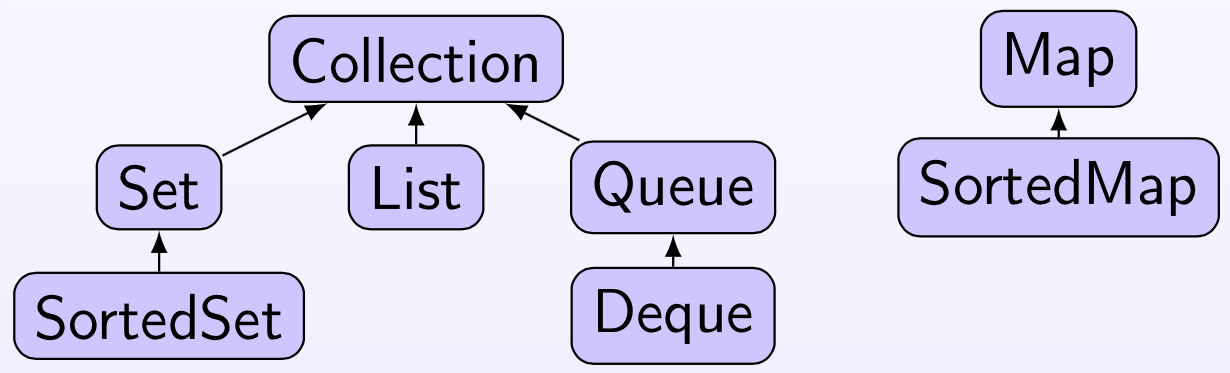
\includegraphics[width=0.5\textwidth]{colls-coreInterfaces.png}
  \caption{Interfacce del  Java collection framework.}
    \label{Fig:collections}
\end{figure}

Ogni interfaccia \`e generica. Quando dichiari una collezione devi specificare il tipo degli oggetti contenuti nella collezione. Questo permette al compilatore di verificare \textbf{a compile time} che il tipo dell'oggetto inserito all'interno di una collezione \`e corretto. Per esempio l'interfaccia \texttt{Collection} \`e specificata come segue, dove \texttt{E} \`e il tipo di elementi contenuti nella collezione.
\begin{lstlisting}
public interface Collection<E>...
\end{lstlisting}
Di seguito vengono specificate le interfacce principali
\begin{itemize}
\item \texttt{Collection}: 
\begin{itemize}
\item rappresenta un gruppo di oggetti (i suoi elementi);
\item l'interfaccia collection \`e la pi\`u generale. Va utilizzata quando un livello massimo di generalit\`a \`e richiesto;
\item non esiste una classe che implementa direttamente collection. 
\end{itemize}
\item \texttt{Set}: 
\begin{itemize}
\item una collezione che \textbf{non} pu\`o contenere elementi duplicati (la presenza di duplicati vine controllata utilizzando i metodo \texttt{hashCode} e \texttt{equals} che devono essere opportunamente reimplementati nella classe che viene sostituita al tipo generico \texttt{E}); 
\item Consente di modellare entit\`a come per esempio un mazzo di carte da briscola (perch\`e non \`e la scelta ideale per un mazzo di carte da scala?) l'insieme di esami sostenuti da uno studente, i processi in esecuzione su una macchina.
\end{itemize} 
\item \texttt{SortedSet}: 
\begin{itemize}
\item un \texttt{Set} che mantiene gli elementi ordinati in ordine ascendente.  
\item \texttt{SortedSet} possono essere utilizzati (per esempio) per memorizzare una insieme ordinato di parole.
\end{itemize}
\end{itemize}
\begin{itemize}
\item \texttt{List}: 
\begin{itemize}
\item \`e una collezione ordinata (a volte chiamata sequenza). 
\item Una lista pu\`o contenere elementi duplicati.
\item  L'utilizzatore di una lista vuole un controlllo preciso su dove un elemento \`e inserito e vuole potervi accedere in base alla sua posizione. 
\item Pu\`o essere utile per esempio al fine di modellizzare l'ordine di arrivo a un gran premio di Formula1.
\end{itemize}
\item \texttt{Queue}: 
\begin{itemize}
\item \`e una collezione utilizzata per modellizzare una coda di elementi  prima che vengano processati. 
\item Una coda \`e in genere implementata (ma non necessariamente) per mezzo di una coda di tipo FIFO (first-in, first-out). 
\item Consente di eseguire operazioni come l'inserimento, l'estrazione o l'ispezione. 
\item Una coda pu\`o essere utilizzata per modellare l'insieme di macchine in coda a un casello autostradale.
\end{itemize}
\item \texttt{Deque}: 
\begin{itemize}
\item viene utilizzata per modellizzare una coda di elementi prima che vengano processati.
\item A differenza della coda, \`e possibile aggiungere e rimuovere gli elementi da entrambi i lati.
\end{itemize}
\item \texttt{Map}: 
\begin{itemize}
\item \`e un oggetto che mappa una chiave in un valore.
\item Una mappa \textbf{non} pu\`o contenere delle chiavi duplicate, 
\item ogni chiave deve essere associata a esattamente un valore (che potrebbe essere un \textbf{Set}). 
\end{itemize}
\item \texttt{SortedMap}: 
\begin{itemize}
\item contiene una mappa dove le chiavi sono mantenute in ordine ascendente. 
\item le mappe ordinate possono essere utilizzate, per esempio, per modellizzare un vocabolario o una guida telefonica.
\end{itemize}
\end{itemize}

Ogni interfaccia fornisce un insieme di metodi. Per esempio l'interfaccia \texttt{Collection} fornisce (tra gli altri) i metodi seguenti:
\begin{itemize}
\item \texttt{boolean	containsAll(Collection<?> c)}: Returns true if this collection contains all of the elements in the specified collection.
\item \texttt{addAll(Collection<? extends E> c)}: Adds all of the elements in the specified collection to this collection (optional operation).
\item \texttt{removeAll(Collection<?> c)}: Removes all of this collection's elements that are also contained in the specified collection (optional operation).
\item \texttt{retainAll(Collection<?> c)}: Retains only the elements in this collection that are contained in the specified collection (optional operation).
\item \texttt{clear()}: Removes all of the elements from this collection (optional operation).
\end{itemize}

\subsubsection{Implementazioni}
Per ogni interfaccia ci sono un insieme di possibili \textbf{implementazioni}. In particolare abbiamo varie implementazioni per vari contesti, tra le quali:
\begin{itemize}
\item \texttt{Implementazioni General-purpose} sono quelle comunemente utilizzate, progettate per l'uso di tutti i giorni
\item \texttt{Implementazioni Special-purpose} sono progettati per usi particolari: garantire performances particolari, restringere l'utilizzo di quelle general purpose.
\item \texttt{Concurrent implementations} sono progettate per supportare applicazioni concorrenti. Queste implementazioni fanno parte del  java.util.concurrent package.
\item \texttt{Wrapper implementations} sono utilizzate in combinazioni con altri tipi di implementazioni per fornire funzionalit\`a aggiunte o ristette.
\end{itemize}

Alcune delle implementazioni General-purpose sono schematizzate nella tabella seguente 

\begin{tabular}{ | l | l | l | l | l | l |}
\hline
  Interfaces & Hash table  & Resizable array  & Tree  & Linked list  & Hash table + Linked list  \\
  \hline
  \texttt{Set} & \texttt{HashSet} &  & \texttt{TreeSet} && \texttt{LinkedHashSet} \\
  \hline
    \texttt{SortedSet} & &  & \texttt{TreeSet} &&  \\
  \hline
  \texttt{List} &  & \texttt{ArrayList}  & & \texttt{LinkedList} & \\
\hline  
  \texttt{Queue} &  & & & \texttt{LinkedList} &  \\
\hline  
  \texttt{Deque} &  & \texttt{ArrayDeque} & & \texttt{LinkedList} & \\
\hline  
  \texttt{Map} & \texttt{HashMap} & & \texttt{TreeMap} && \texttt{LinkedHashMap} \\
  \hline
    \texttt{SortedMap} & & & \texttt{TreeMap} &&  \\
\hline    
\end{tabular} 

Ognuna di queste implementazioni:
\begin{itemize}
\item permette elementi \texttt{null} (sia per chiavi che per valori)
\item non \`e sincronizzata (thread-safe): non adatta quando thread concorrenti devono modificare la collezione
\item ha degli itaratori \emph{fail-fast} lanciano un eccezione quando viene eseguita una modica durante un iterazione. 
\item sono tutte serializzabili
\item hanno tutte un metodo clone (nota il metodo clone non clona gli elementi ma solo i loro references)
\end{itemize}

\begin{framed}
Come regola \`e bene pensare in termini di interfacce e non di implementazioni. Nella maggior parte dei casi l'implementazione influenza solo le performances. \`E bene associare un implementazione direttamente alla sua interfaccia (nella fase di instanziazione) e specificare come parametri di ingresso o uscita dei metodi solamente interfacce, lasciando il programmatore libero di cambiare implementazione a suo piacimento. 
\end{framed}

\subsubsection{Algoritmi}
Molti degli algoritmi forniti dal Java collection framework sono forniti dalla classe \texttt{Collections}. In particolare, questi metodi sono implementati come dei metodi \texttt{static} il cui primo parametro \`e la collezione su cui il metodo deve essere eseguito. La maggior parte dei metodi agisce su parametri di tipo \texttt{List} ma esistono anche metodi che lavorano su \texttt{Collection} generiche.
Tra gli altri sono forniti algoritmi di 
\begin{itemize}
\item Sorting: forniscono dei metodi per ordinare una lista
\item Shuffling: permettono di mischiare gli elementi presenti in una lista
\item Routine Data Manipulation: cercano, scambiano, copiano degli elementi
\item Searching: ricercano elementi specifici nella collezione
\item Composition: permettono di sapere il numero di volte che un elemento \`e resente o quando due collezioni non hanno elementi in comune
\item Finding Extreme Values: ritornano il minimo o il massimo valore presente in una collezione
\end{itemize}









\subsubsection{Conversione tra collezioni}
Ogni collezione ha un costruttore (detto \emph{conversion constructor}) che prende come parametro una collezione. \`E possibile usare questo costruttore per convertire una collezione di un tipo in un'altra collezione di un altro tipo.
\begin{lstlisting}
List<String> ls=new ArrayList<String>();
Set<String> lo=new HashSet<String>(ls);
\end{lstlisting}

\subsubsection{Conversione tra array e collezioni}
\`E possibile convertire un array in una collezione e viceversa.
\begin{itemize}
\item da collection a array: per convertire un array in una collezione \`e possibile utilizzare il metodo \texttt{toArray()} specificata nell'interfaccia \texttt{List}
\begin{lstlisting}
List<String> miaLista=new ArrayList<String>();
String[] array=miaLista.toArray();
\end{lstlisting}
\end{itemize}
\begin{itemize}
\item da array a collection: per convertire da un array a una collezione si pu\`o utilizzare il metodo \texttt{statico} \texttt{asList} della classe \texttt{Array}.
\begin{lstlisting}
String[] stringArray = new String[20];
List<String> miaList=Arrays.asList(stringArray);
Set<String> mioSet=new HashSet<String>(miaList);
\end{lstlisting}
\end{itemize}


\subsubsection{Iterazione}
Per eseguire delle iterazioni su una collezione ci sono due possibili modi:
\begin{itemize}
\item for generalizzato:
\begin{lstlisting}
Collection<String> collezione=new HashSet<String>();
for(String s: collezione){
    System.out.println(s);
}
\end{lstlisting}
\item iteratore:
\begin{lstlisting}
Collection<String> collezione=new HashSet<String>();
Iterator<String> it=c.iterator;
while(it.hasNext()){
    System.out.println(it.next());
}
\end{lstlisting}
\end{itemize}


\section{Esercizi}

\subsection{Generics}
\subsubsection{Generic classes}
\Esercizio{Pregettare la classe \texttt{Box}. La classe \texttt{Box} contiene un oggetto e fornisce il metodo \texttt{set}, che modifica l'oggetto contenuto nel box, e  \texttt{get}, che ottiene l'oggetto contenuto nel \texttt{Box}.}

\begin{lstlisting}[language=Java]
public class Box {
    private Object object;

    public void set(Object object) { this.object = object; }
    public Object get() { return object; }
}
\end{lstlisting}
Dal momento che i metodi accettano e ritornano un oggetto di tipo \texttt{Object}, l'utente \`e libero di passare qualunque dato non sia primitivo. Non c'\`e modo di verificare a \emph{compile time} come la classe viene usata. Per esempio uno sviluppatore potrebbe usare in una parte di codice il Box come un box di interi, ma poi ``dimenticarsene" e in un altra parte passagli una stringa. Tale comportamento genera un errore a \emph{run time}. Per esempio il seguente snapshot genera un errore a run-time 
\begin{lstlisting}[language=Java]
public class Main {

	public static void main(String[] args) {
		Box b1=new Box();
		b1.set("1");
		String stringNumber=(String) b1.get();
		int number=(int) b1.get();
	}
}
\end{lstlisting}
In seguito viene descritta l'implementazione del box eseguita mediante l'utilizzo dei generici. Specifichiamo che la classe pu\`o contenere oggetti di un tipo \emph{generico} \texttt{T}. 

\begin{lstlisting}[language=Java]
/*
 * Generic version of the Box class.
 * @param <T> the type of the value being boxed
 */
public class Box<T> {
    // T stands for "Type"
    private T t;

    public void set(T t) { this.t = t; }
    public T get() { return t; }
}
\end{lstlisting}
Nel seguito viene descritto un possibile utilizzo della classe \texttt{Box}, un \texttt{Box} contenente una stringa. Analogamente \`e possibile dichiarare un \texttt{Box} contenente una bicicletta come \texttt{Box<Bicicletta>}.
\begin{lstlisting}[language=Java]
public class Main {

	public static void main(String[] args) {
		Box<String> b1=new Box<String>();
		b1.set("1");
		b1.set(1); // errore a compile time
		String stringNumber= b1.get();
		int number=b1.get(); 
		// errore a compile time
	}
}
\end{lstlisting}

\subsubsection{Generic methods}
\Esercizio{Pregettare una classe \texttt{Utils}, contenente un metodo che dati due \texttt{Box} ritorna \texttt{true} se entrambi i box sono vuoti, \texttt{false} altrimenti}

Prima di tutto aggiungiamo il metodo \texttt{isEmpty()} alla classe box
\begin{lstlisting}[language=Java]
public boolean isEmpty(){
    		return (t==null);
    }
\end{lstlisting}

Definiamo il metodo \texttt{check} i cui parametri sono due \texttt{Box} che contengono un elemento di tipo \texttt{K} e \texttt{V}, rispettivamente, il cui comportamento rispetta i requisiti richiesti.
\begin{lstlisting}[language=Java]
public final class Utils {

	public static <K, V>  boolean check(Box<K> box1, Box<V> box2){
		return box1.isEmpty()&&box2.isEmpty();
	}
}
\end{lstlisting}
Specifichiamo un client che utilizza il metodo \texttt{check}
\begin{lstlisting}[language=Java]
public class Main {

	public static void main(String[] args) {
		Box<String> b1=new Box<String>();
		b1.set("1");
		Box<String> b2=new Box<String>();
		b2.set("1");
		Box<Integer> b3=new Box<Integer>();
		Box<String> b4=new Box<String>();
		System.out.println(Utils.<String, String>check(b1, b2));
		System.out.println(Utils.<String, String>check(b1, b2));
		System.out.println(Utils.<Integer, String>check(b3, b4));
	}
}
\end{lstlisting}

\subsubsection{Generic Bounded types}
\Esercizio{Pregettare la classe \texttt{Box}. La classe \texttt{Box} contiene un oggetto di tipo \textbf{animale} o suoi sottotipi. La classe fornisce il metodo \texttt{set}, che modifica l'oggetto contenuto nel box, e  \texttt{get}, che ottiene l'oggetto contenuto nel \texttt{Box}.}

E\` possibile specificare che il tipo generico sostituito a \texttt{T} debba estendere una classe o implementare un interfaccia. Nel caso in questione forziamo \texttt{T} a estendere la classe \texttt{Animale}.

\begin{lstlisting}[language=Java]
/*
 * Generic version of the Box class.
 * @param <T> the type of the value being boxed
 */
public class Box<T extends Animale> {
    // T stands for "Type"
    private T t;

    public void set(T t) { this.t = t; }
    public T get() { return t; }
    
    public boolean isEmpty(){
    		return (t==null);
    }
}
\end{lstlisting}

Di seguito viene specificato un client per la nuova classe \texttt{Box}

\begin{lstlisting}[language=Java]
public class Main {

	public static void main(String[] args) {
		Box<Animale> b1=new Box<Animale>();
		b1.set(new Cane());
		System.out.println(b1.get());
		Box<String> b2=new Box<String>(); // ERRORE COMPILAZIONE
	}
}
\end{lstlisting}

\subsubsection{Wildcard}
\Esercizio{Scrivere un metodo che stampa gli elementi di una collection di qualsiasi tipo.}

La prima soluzione che potrebbe venirci in mente \`e la seguente: dichiarare un metodo che prende come parametro una collezione di elementi il cui tipo \`e \texttt{Object}.
\begin{lstlisting}[language=Java]
void printCollection(Collection<Object> c){
    for(Object e: c){
        System.out.println(e);    
    }
}
\end{lstlisting}
 Tuttavia questa soluzione non ci pemette di stampare una collezione di \texttt{String}. Infatti, bench\`e \texttt{String} estende \texttt{Object} non \`e vero che \texttt{Collection<Object>} estende \texttt{Collection<String>}. Quindi non \`e possibile chiamare il metodo \texttt{printCollection} passando come parametro una \texttt{Collection<String>}.

La soluzione seguente risolve il problema: prende come parametro una \texttt{Collection}, ma il tipo degli elementi presenti nella \texttt{Collection} non \`e di interesse. \`E possibile passare al metodo una collection arbitraria.
\begin{lstlisting}[language=Java]
void printCollection(Collection<?> c){
    for(Object e: c){
        System.out.println(e);    
    }
}
\end{lstlisting}

\subsubsection{Bounded Wildcard}
\Esercizio{Aggiungere un metodo \texttt{drawAll} in ShapeClient per disegnare tutte le figure di una lista di figure}

La prima soluzione a cui possiamo pensare \`e la seguente:
\begin{lstlisting}[language=Java]
void drawAll(List<Shape> shapes) { 
    for (Shape s : shapes) {
        s.draw(this); 
    }
}
\end{lstlisting}
Tuttavia il problema \`e il medesimo a quello precedentemente descritto: non \`e possibile passare come parametro al metodo \texttt{drawAll} una lista di \texttt{Circle} (\texttt{List<Circle>}). Potremmo utilizzare una soluzione equivalemente a quella espressa nel metodo \texttt{printCollection}, ma sarebbe troppo generica: sarebbe possibile stampere oggetti che non sono \texttt{Shape}. La soluzione \`e utilizzare un \texttt{Bound} (limite) all'operatore \texttt{Shape}, come specificato nel seguente metodo.
\begin{lstlisting}[language=Java]
void drawAll(List<? extends Shape> shapes) { 
    for (Shape s : shapes) {
        s.draw(this); 
    }
}
\end{lstlisting}



\subsection{Collezioni}

\subsubsection{Liste assegnamenti}
\Esercizio{Dire se sono valide le seguenti operazioni}

\begin{lstlisting}
List<String> ls=new ArrayList<String>();
List<Object> lo=ls;
\end{lstlisting}

La prima istruzione \`e certamente corretta. La classe \texttt{ArrayList} implementa l'interfaccia \texttt{List}, e il tipo specificato per il parametro generico \`e il medesimo. La seconda istruzione non \`e corretta: bench\`e \texttt{String} estende \texttt{Object}, una lista di \texttt{String} non estende una lista di \texttt{Object}. Il compilatore genera un errore.l


\subsubsection{Rimozione di duplicati}
\Esercizio{Scrivere un metodo statico che data una collezione di \texttt{String} rimuove i duplicati e stampa il numero di elementi non duplicati e i corrispettivi elementi}

Nella prima versione della soluzione utilizziamo il for generalizzato
\begin{lstlisting}
package es1;

import java.util.ArrayList;
import java.util.Collection;
import java.util.HashSet;
import java.util.List;
import java.util.Scanner;
import java.util.Set;

public class FindDups {
	public static void findDups(Collection<String> words){
		Set<String> set = new HashSet<String>();
		for (String s: words){
			set.add(s);
		}
		System.out.println("Unique values, dim : " + 
		set.size() + " Elements:" + set);
			
	}
}
\end{lstlisting}

Nella seconda versione utilizziamo direttamente il costruttore di \texttt{HashSet} vedi (\url{https://docs.oracle.com/javase/6/docs/api/java/util/HashSet.html}). In generale \`e sempre utile consultare la Javadoc degli elementi per controllare che le funzionalit\`a che dobbiamo sviluppare non siano gi\`a state implementate.
\begin{lstlisting}
package collections;

import java.util.Collection;
import java.util.HashSet;
import java.util.Set;

public class FindDups {
	public static void findDups(Collection<String> words){
		Set<String> set = new HashSet<String>(words);
		System.out.println("Unique values, dim : " + 
				set.size() + " Elements:" + set);
		
	}
}
\end{lstlisting}
Di seguito viene riportato un client per la classe \texttt{FindDups}.
\begin{lstlisting}
	public static void main(String[] args){
		Scanner s = new Scanner(System.in);
		String word = null;
		System.out.println("Inserire le parole, (q per uscire)");
		List<String> words = new ArrayList<String>();
		word = s.nextLine();		
		while (!word.equals("q") ){
			words.add(word);
			word = s.nextLine();
		} 
		findDups(words);
		s.close();
	}
}
\end{lstlisting}

\subsubsection{Shuffle}
\Esercizio{Scrivere un metodo statico che data una permette di mescolare degli oggetti contenuti in una lista.}

Nella prima versione implementiamo la funzione shuffle 
\begin{lstlisting}
package collections;

import java.util.List;
import java.util.Random;

public class Shuffle {
	public static <E> void swap(List<E> a, int i, int j) {
		    E tmp = a.get(i);
		    a.set(i, a.get(j));
		    a.set(j, tmp);
	}
	
	public static void shuffle(List<Integer> list, Random rnd) {
		    for (int i = list.size(); i > 1; i--)
		        swap(list, i - 1, rnd.nextInt(i));
	}
}
\end{lstlisting}
Ecco il corrispettivo client
\begin{lstlisting}
public class Main {

	public static void main(String[] args){
		List<Integer> list = new ArrayList<Integer>();
		for (int i = 0; i < 10; i++){
			list.add(i);
		}
		System.out.println(list);
		Shuffle.shuffle(list, new Random());
		System.out.println(list);
	}
}
\end{lstlisting}
Nella seconda versione utilizziamo il metodo \texttt{shuffle} contenuto nella classe \texttt{Collections}.

\begin{lstlisting}
public class Shuffle {
	public static void shuffle(List<Integer> list) {
		Collections.shuffle(list);
	}
}
\end{lstlisting}
Ecco il corrispondente client
\begin{lstlisting}
package collections;

import java.util.ArrayList;
import java.util.List;

public class Main {

	public static void main(String[] args){
		List<Integer> list = new ArrayList<Integer>();
		for (int i = 0; i < 10; i++){
			list.add(i);
		}
		System.out.println(list);
		Shuffle.shuffle(list);
		System.out.println(list);
	}
}
\end{lstlisting}


\subsubsection{Number of tokens}
\Esercizio{Scrivere un metodo statico che data una stringa conta il numero di occorrenze di ogni parola. Suggerimento: controllare la Javadoc della classe \texttt{StringTokenizer}}

\begin{lstlisting}
public static void count(String text){
    StringTokenizer tokenizer = 
        new StringTokenizer(text);
    Map<String,Integer> frequencyCounterMap = 
        new HashMap<String,Integer>();
    while (tokenizer.hasMoreTokens()){
        String word = tokenizer.nextToken();
        Integer freq = frequencyCounterMap.get(word);
        frequencyCounterMap.put(word,
            (freq == null) ? 1 : freq + 1);
    }
    System.out.println(frequencyCounterMap.size() +
         " parole distinte");
    System.out.println(frequencyCounterMap);
}
\end{lstlisting}



%\subsection{Stack}
%
%
%
%\subsubsection{Node}
%\begin{lstlisting}
%/**
%* contiene un nodo dello stack. 
%* Un nodo contiene un reference al prossimo nodo (next)
%* e l'elemento corrente (element)
%*/
%class Node<E> {
%    /**
%    * contiene il reference al prossimo elemento
%    */	
%    Node<E> next;
%    /**
%    * contiene l'elemento contenuto nel nodo
%    */
%    E element;
%}
%\end{lstlisting}
%
%\subsubsection{Stack}
%\begin{lstlisting}
%import java.util.Collection;
%
%/**
%* contiene l'interfaccia che definisce le operazioni consentite dallo stack
%*/
%public interface MyStack <E>{
%    /**
%    * rimuove un elemento dal top dello stack
%    */
%    public E pop();
%    /**
%    * inserisce un elemento nello stack
%    */
%    public void push(E elem);
%    /**
%    * ritorna vero se lo stack e' vuoto
%    */
%    public boolean isEmpty();
%    /**
%    * ritorna la dimensione dello stack
%    */
%    public int size();
%    /**
%    * ritorna vero se l'elemento e' contenuto nello stack
%    */
%    public boolean contains(E elem);
%    /**
%    * ritorna vero se lo stack contiene tutti gli elementi della collezione
%    */
%    public boolean containsAll(Collection<? extends E> collection);
%}
%\end{lstlisting}
%
%\subsection{LinkedListStack}
%\begin{lstlisting}
%import java.util.Collection;
%
%public class LinkedListStack<E> implements MyStack<E>{
%	private int N;
%	private Node<E> head;
%
%	public LinkedListStack(){
%		head = null;
%		N = 0;
%	}
%	
%	@Override
%	public E pop() {
%		if (isEmpty())
%			return null;
%		E elem = head.element;
%		head = head.next;
%		N--;
%		return elem; 
%	}
%
%	@Override
%	public void push(E elem) {
%		Node<E> oldHead = head;
%		head = new Node<E>();
%		head.element = elem;
%		head.next = oldHead;
%		N++;		
%	}
%
%	@Override
%	public boolean isEmpty() {		
%		return N == 0;
%	}
%
%	@Override
%	public boolean contains(E elem) {
%		Node<E> tmp = head;
%		while (tmp!= null){
%			if (tmp.element.equals(elem))
%				return true;
%			tmp = tmp.next;
%		}
%		return false;
%	}
%
%	@Override
%	public boolean containsAll(Collection<? extends E> collection) {		
%		for (E elem: collection){
%			if (!contains(elem))
%				return false;			
%		}
%		return true;
%	}
%	
%	@Override
%	public int size(){
%		return N;
%	}
%	
%	public static <E> MyStack<E> createFromArray(E[] arr){
%		MyStack<E>	stack = new LinkedListStack<>();
%		for (E elem: arr){
%			stack.push(elem);
%		}
%		return stack;
%	}
%
%	
%	public static void main(String[] args){
%		String [] arr = {"a","b","c","d"};
%		MyStack<String> stack = createFromArray(arr);
%		System.out.println(stack.contains("c"));
%		System.out.println(stack.contains("f"));
%		stack.push("e");
%		while (!stack.isEmpty()){
%			System.out.println(stack.pop());
%		}
%	}
%}
%\end{lstlisting}

\section{Esercizi per casa}
\begin{itemize}
\item Generici
\begin{itemize}
\item implementare la classe coppia, che rappresenta una coppia di elementi. I due elementi hanno dei tipi generici \texttt{K}, \texttt{V}.
\item progettare un metodo statico che date due coppie i cui elementi sono dello stesso tipo ritorna true se le coppie rappresentano il medesimo oggetto
\end{itemize} 
\item Collezioni
\begin{itemize}
\item modificare il gioco degli scacchi utilizzando le collezioni in modo opportuno al fine di memorizzare le mosse eseguite dai due giocatori al fine di mostrare al termine della partita  il log delle mosse (la ``storia della partita").
\end{itemize}
\end{itemize}


\clearpage

% ---- Bibliography ----




\addcontentsline{toc}{chapter}{Bibliography}
\bibliographystyle{alpha}
\bibliography{bib}
\nocite{*}


\end{document}

